\documentclass[11pt,a4paper]{article}

% --- Packages ---
\usepackage[utf8]{inputenc}
\usepackage[margin=1in,headheight=14pt]{geometry}
\usepackage{graphicx}
\usepackage{xcolor}
\usepackage{tikz}
\usetikzlibrary{positioning, arrows.meta, calc, shapes.geometric}
\usepackage{url}
\usepackage{hyperref}
\usepackage{booktabs}
\usepackage{tabularx}
\usepackage{multirow}
\usepackage{subcaption}
\usepackage{amsmath}
\usepackage{amssymb}
\usepackage{fancyhdr}
\usepackage{titlesec}
\usepackage{enumitem}
\usepackage{tcolorbox}
\tcbuselibrary{skins, breakable}
\usepackage{listings}
\usepackage{microtype}
\usepackage{placeins}
\usepackage{ragged2e}

\urlstyle{tt}
\newcommand{\filepath}[1]{\path{#1}}
\newcolumntype{Y}{>{\RaggedRight\arraybackslash}X}
\setlength{\emergencystretch}{2em}

% --- Safe Screenshot Insertion Macro (Supports both Overleaf preview and uploaded images) ---
\newcommand{\screenimage}[3]{%
  \IfFileExists{#3}{%
    \includegraphics[width=#1]{#3}%
  }{%
    \fbox{\begin{minipage}[c][#2][c]{#1}
      \centering\small
      Screenshot pending\\[4pt]
      \filepath{#3}
    \end{minipage}}%
  }%
}

% --- Color Palette (All Text set to Professional Black as requested) ---
\definecolor{DishDashRed}{HTML}{E53935}
\definecolor{ObsidianOnyx}{HTML}{161622}
\definecolor{SoftBackground}{HTML}{F8F9FC}
\definecolor{TextPrimary}{HTML}{000000}
\definecolor{BorderGray}{HTML}{CCCCCC}
\definecolor{BoxBg}{HTML}{F8F9FA}

% --- Hyperref Setup (Clean Black Links for Professional Printing) ---
\hypersetup{
    colorlinks=true,
    linkcolor=black,
    citecolor=black,
    urlcolor=black,
    pdftitle={DishDash Restaurant Ordering Experience - Technical Product Report},
    pdfauthor={Maryam},
    pdfsubject={Flutter Cross-Platform Food Ordering Application Documentation}
}

% --- Header and Footer ---
\pagestyle{fancy}
\fancyhf{}
\rhead{\textcolor{black}{\small DishDash -- Technical Product Report}}
\lhead{\textcolor{black}{\small Flutter Internship Submission}}
\rfoot{\textcolor{black}{\small Page \thepage}}
\lfoot{\textcolor{black}{\small Prepared by Maryam}}
\renewcommand{\headrulewidth}{0.4pt}
\renewcommand{\footrulewidth}{0.4pt}

% --- Section Styling (Professional Black Headings) ---
\titleformat{\section}
  {\normalfont\Large\bfseries\color{black}}{\thesection}{1em}{}[\titlerule]
\titleformat{\subsection}
  {\normalfont\large\bfseries\color{black}}{\thesubsection}{1em}{}
\titleformat{\subsubsection}
  {\normalfont\normalsize\bfseries\color{black}}{\thesubsubsection}{1em}{}

% --- Code Listing Styling (Strict Line Wrapping) ---
\lstset{
  backgroundcolor=\color{SoftBackground},
  basicstyle=\ttfamily\small\color{black},
  breaklines=true,
  breakatwhitespace=false,
  captionpos=b,
  commentstyle=\color{gray},
  keywordstyle=\bfseries\color{black},
  stringstyle=\color{black},
  frame=single,
  rulecolor=\color{BorderGray},
  showstringspaces=false
}

% --- Custom Callout Boxes for Notes ---
\newtcolorbox{notebox}[1][Note]{
  colback=BoxBg,
  colframe=black,
  fonttitle=\bfseries\color{white},
  title={#1},
  arc=3pt
}

\begin{document}
\hypersetup{pageanchor=false}

% ==============================================================================
% TITLE PAGE (Clean Executive Design with Perfect Fit Box)
% ==============================================================================
\begin{titlepage}
    \centering
    \vspace*{1.0cm}
    
    {\Huge \bfseries DishDash} \\[0.4cm]
    {\Large \textbf{Restaurant Ordering Experience}} \\[0.6cm]
    
    \rule{\linewidth}{1.5pt} \\[1.2cm]
    
    {\Large \textit{Technical Product Report}} \\[0.3cm]
    {\large Interaction Flow, Engineering Decisions, Responsive Delivery, \\ and Feature Validation} \\[2.0cm]
    
    \vfill
    
    \begin{tcolorbox}[colback=white, colframe=black, width=\linewidth, arc=4pt, boxrule=1.2pt]
        \vspace{2mm}
        \small
        \begin{tabularx}{\linewidth}{@{}l X@{}}
            \textbf{Experience:} & DishDash Restaurant Ordering Platform \\[3pt]
            \textbf{Technology Base:} & Flutter and Dart SDK $\ge$ 3.10 \\[3pt]
            \textbf{Application State:} & Provider with \texttt{ChangeNotifier} \\[3pt]
            \textbf{Delivery Surfaces:} & Android, iOS, Tablet, and Desktop Web \\[3pt]
            \textbf{Submission:} & Responsive Frontend and Engineering Report \\[3pt]
            \textbf{Author:} & Maryam, Flutter Development Intern \\[3pt]
            \textbf{Host Organization:} & Verxeon Technologies \\[3pt]
            \textbf{Issued:} & July 29, 2026 \\
        \end{tabularx}
        \vspace{2mm}
    \end{tcolorbox}
    
    \vspace*{0.8cm}
\end{titlepage}
\hypersetup{pageanchor=true}
\pagenumbering{roman}

% ==============================================================================
% TABLE OF CONTENTS
% ==============================================================================
\newpage
\tableofcontents
\newpage
\pagenumbering{arabic}

% ==============================================================================
% 1. EXECUTIVE SUMMARY
% ==============================================================================
\section{Project Overview}

\textbf{DishDash} is a premium, cross-platform food ordering application built with the \textbf{Flutter} framework and \textbf{Provider} state management system as part of the Verxeon internship task. The application delivers an end-to-end digital restaurant experience, allowing customers to seamlessly explore interactive food categories, apply multi-criteria filtering, customize dishes with gourmet add-ons and dietary preferences, manage a dynamic shopping cart, execute checkout flows, track live order status through real-time background simulation, and store personal favorite dishes.

Developed completely on the client-side with a 100\% decoupled local mock data layer (\texttt{lib/\allowbreak data/}), DishDash functions without external server or database dependencies, making it instantly deployable for client demonstrations, testing, and rapid white-label customization. The codebase adheres strictly to enterprise Flutter architecture standards, ensuring that a live backend (such as Firebase, Supabase, or a custom REST API) can be integrated with minimal refactoring to the presentation and provider layers.

This document details the business context, architectural decisions, design token system, state management mechanics, responsive layout strategy, screen-by-screen functionality, quality assurance matrix, and future expansion roadmap.

\FloatBarrier

% ==============================================================================
% 2. PROJECT BACKGROUND
% ==============================================================================
\section{Business Context}

The modern food delivery and restaurant industry demands highly responsive, visually appealing digital touchpoints. Traditional single-platform applications often suffer from fragmented UI experiences across devices, bloated codebases, and poor state synchronization between cart items, order tracking, and user favorites.

Common challenges encountered in early-stage restaurant app development include:
\begin{itemize}[leftmargin=*]
    \item \textbf{UI Inconsistency Across Breakpoints:} Inability to adapt gracefully between mobile portrait screens, medium tablet viewports, and wide desktop web browsers.
    \item \textbf{Complex State Management:} High friction when updating cart counters, calculating taxes/discounts dynamically, and sharing order status updates across unrelated screens.
    \item \textbf{Lack of Re-Branding Flexibility:} Hardcoded assets and color schemes that prevent white-label reuse for different restaurant clients.
    \item \textbf{Janky Scrolling \& Asset Overhead:} Performance degradation during list scrolling due to unoptimized network image rendering.
    \item \textbf{Static Mock Simulations:} Difficulty demonstrating live features (e.g., live delivery status timelines) without an active backend server.
\end{itemize}

The DishDash project was engineered specifically to solve each of these challenges through modular component architecture, centralized reactive state management, adaptive responsive wrappers, and background timer-based status simulations.

\FloatBarrier

% ==============================================================================
% 3. PROJECT OBJECTIVES & SCOPE
% ==============================================================================
\section{Project Scope and Objectives}

The primary objectives achieved during the development of DishDash were:
\begin{enumerate}[leftmargin=*]
    \item \textbf{Complete Customer Journey:} Construct a fully functional, multi-screen user flow: 
    \begin{center}
    \small\bfseries
    Splash $\longrightarrow$ Home $\longrightarrow$ Menu \& Filters $\longrightarrow$ Food Customization \\
    $\longrightarrow$ Cart $\longrightarrow$ Checkout $\longrightarrow$ Live Order Stepper
    \end{center}
    \item \textbf{Reactive State Architecture:} Implement centralized \texttt{ChangeNotifier} providers for Cart, Favourites, Filter Criteria, and Orders.
    \item \textbf{Adaptive Responsive Layout Engine:} Ensure the application renders optimally across Mobile ($<650\text{px}$), Tablet ($650\text{px} - 1100\text{px}$), and Desktop Web ($\ge 1100\text{px}$) form factors using custom header app bars, mobile navigation bars, and tablet drawers.
    \item \textbf{Live Order Tracking Simulation:} Feature an automated background status timer (\texttt{Timer.periodic}) that advances order status through realistic lifecycle stages:
    \begin{center}
    \small\bfseries
    Placed $\longrightarrow$ Preparing $\longrightarrow$ Ready $\longrightarrow$ On the way $\longrightarrow$ Delivered
    \end{center}
    \item \textbf{Gourmet Design System:} Establish a cohesive visual design token hierarchy (\textbf{Gourmet Crimson Red} and \textbf{Obsidian Onyx}) with Google Fonts (\textbf{Poppins}), elevation shadows, and custom dietary badges (\textbf{VEG}, \textbf{SPICY}).
    \item \textbf{White-Label Architecture:} Decouple data and style tokens so third-party restaurant clients can rebrand the platform by editing only two configuration files.
\end{enumerate}

\FloatBarrier

% ==============================================================================
% 4. SOLUTION ARCHITECTURE
% ==============================================================================
\section{System Architecture}

DishDash follows a modular, layered architecture that emphasizes separation of concerns, scalability, maintainability, and platform independence. Each architectural layer is responsible for a specific set of tasks and communicates cleanly with adjacent layers.

The application is organized around five collaborating areas: the customer-facing screens, responsive routing shell, shared Provider state, local models and repositories, and the reusable visual system. Figure~\ref{fig:architecture} shows how information moves between them.

\begin{figure}[htbp]
\centering
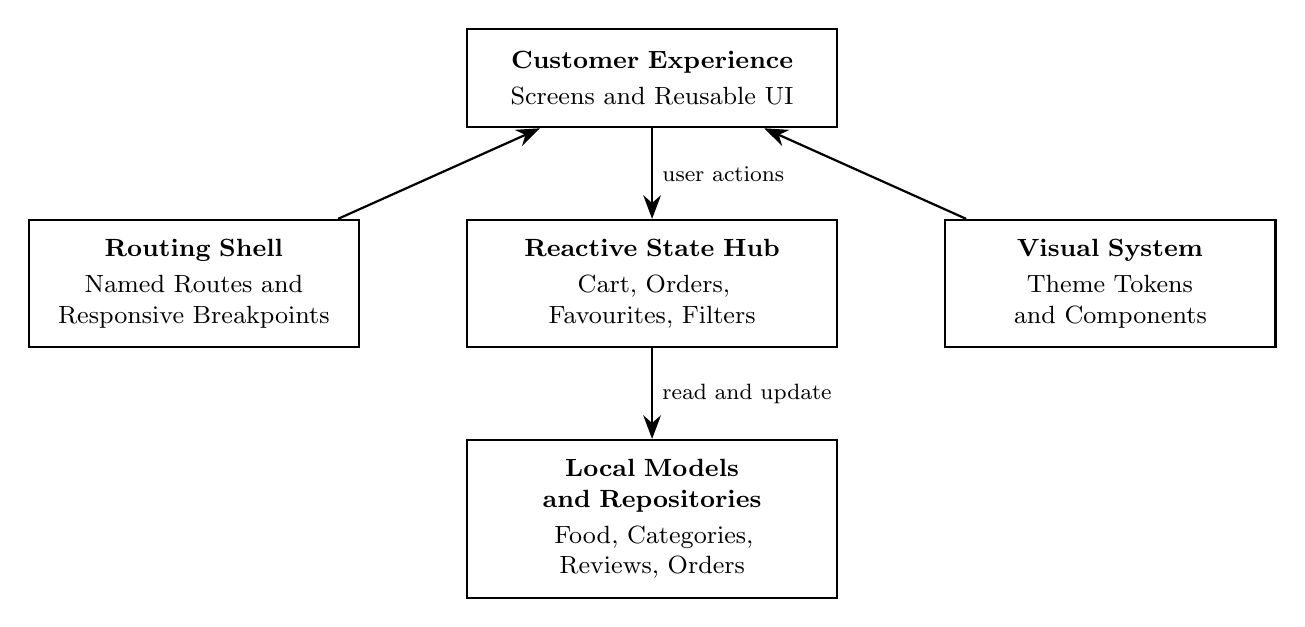
\begin{tikzpicture}[
    node distance=1.15cm and 1.35cm,
    flowbox/.style={
        rectangle,
        draw=black,
        fill=white,
        thick,
        align=center,
        minimum height=1.25cm,
        text width=4.2cm,
        inner sep=7pt,
        font=\small
    },
    sidebox/.style={flowbox, text width=3.7cm},
    flowarrow/.style={-{Stealth[length=3mm]}, thick, draw=black}
]

\node[flowbox] (screens) {
    \textbf{Customer Experience}\\[2pt]
    Screens and Reusable UI
};

\node[flowbox, below=of screens] (state) {
    \textbf{Reactive State Hub}\\[2pt]
    Cart, Orders, Favourites, Filters
};

\node[flowbox, below=of state] (data) {
    \textbf{Local Models and Repositories}\\[2pt]
    Food, Categories, Reviews, Orders
};

\node[sidebox, left=of state] (routing) {
    \textbf{Routing Shell}\\[2pt]
    Named Routes and Responsive Breakpoints
};

\node[sidebox, right=of state] (design) {
    \textbf{Visual System}\\[2pt]
    Theme Tokens and Components
};

\draw[flowarrow] (routing) -- (screens);
\draw[flowarrow] (design) -- (screens);
\draw[flowarrow] (screens) -- node[right, font=\footnotesize] {user actions} (state);
\draw[flowarrow] (state) -- node[right, font=\footnotesize] {read and update} (data);

\end{tikzpicture}
\caption{DishDash Application Interaction Flow}
\label{fig:architecture}
\end{figure}

\begin{table}[htbp]
\caption{Responsibilities Across the DishDash Flow}
\label{tab:architecture_components}
\centering
\small
\begin{tabularx}{\linewidth}{@{}l X@{}}
\toprule
\textbf{Architecture Layer} & \textbf{Technical Responsibilities} \\
\midrule
\textbf{Presentation Layer} & Contains UI screens (\texttt{lib/\allowbreak screens/}) and atomic reusable widgets (\texttt{lib/\allowbreak components/}). Responsible solely for rendering views based on Provider state. \\
\addlinespace
\textbf{Navigation Layer} & Centralized routing via \texttt{AppRouter} using named routes. \texttt{MainLayout} injects bottom bars (mobile), drawers (tablet), or header bars (desktop). \\
\addlinespace
\textbf{State Management Layer} & Global state handled via \texttt{Provider} and \texttt{ChangeNotifier}. Manages cart calculations, live status simulation timers, filtering, and favorites. \\
\addlinespace
\textbf{Data Layer} & Immutable Dart models (\texttt{FoodItem}, \texttt{Order}, \texttt{Category}) backed by single-source-of-truth mock repositories (\texttt{lib/\allowbreak data/}). \\
\addlinespace
\textbf{Design System Layer} & Centralized themes in \texttt{AppTheme} and \texttt{AppColors} controlling Poppins typography, Material 3 color roles, soft shadows, and card radii. \\
\bottomrule
\end{tabularx}
\end{table}

\FloatBarrier

% ==============================================================================
% 5. TECHNOLOGY STACK
% ==============================================================================
\section{Technology and Dependencies}

The application leverages Flutter's high-performance rendering engine alongside production-tested Dart packages listed in Table~\ref{tab:tech_stack}.

\begin{table}[htbp]
\caption{Runtime Tools and Supporting Packages}
\label{tab:tech_stack}
\centering
\small
\begin{tabularx}{\linewidth}{@{}lllX@{}}
\toprule
\textbf{Package / Tool} & \textbf{Version} & \textbf{Type} & \textbf{Usage \& Purpose} \\
\midrule
\textbf{Flutter SDK} & $\ge 3.10.7$ & Framework & Core cross-platform engine targeting iOS, Android, and Desktop Web. \\
\textbf{Dart SDK} & $\ge 3.0.0$ & Language & Object-oriented, sound null-safe programming language. \\
\textbf{provider} & \texttt{\^{}6.1.2} & Dependency & Reactive state management for cart, filters, orders, and favorites. \\
\textbf{google\_fonts} & \texttt{\^{}6.2.1} & Dependency & Delivers clean Poppins typography across headlines and body copy. \\
\textbf{cupertino\_icons} & \texttt{\^{}1.0.8} & Dependency & iOS-style icons for cross-platform fidelity. \\
\textbf{flutter\_lints} & \texttt{\^{}6.0.0} & Dev Dep & Enforces strict Dart style rules and code cleanliness. \\
\bottomrule
\end{tabularx}
\end{table}

\FloatBarrier

% ==============================================================================
% 6. APPLICATION ARCHITECTURE & FOLDER STRUCTURE
% ==============================================================================
\section{Codebase Organization}

The repository is structured according to domain separation of concerns, keeping visual components, business logic, routing, and data mock layers isolated.

\begin{lstlisting}[caption={DishDash Codebase Directory Layout}]
lib/
|-- assets/             # Images, brand logos, food thumbnails & illustrations
|-- components/         # Atomic reusable UI widgets
|   |-- app_bar/        # Responsive header bar (CustomAppBar)
|   |-- bottom_nav/     # Floating mobile navigation bar (CustomBottomNavBar)
|   |-- buttons/        # Standard primary, secondary, and icon buttons
|   |-- category_card/  # Category selection chips & cards
|   |-- custom_banner/  # Hero banner carousel widget
|   |-- filters/        # Advanced multi-criteria Filter Panel
|   |-- food_card/      # Reusable Food Card (Grid & List views)
|   |-- footer/         # Comprehensive global footer
|   |-- loader/         # Skeleton shimmer loaders
|   |-- modal/          # Reusable dialogs & image zoom modal
|   |-- search_bar/     # Search input bar with quick filters
|   `-- testimonials/   # Customer review cards & rating stars
|-- data/               # Single-source-of-truth mock dataset
|   |-- mock_categories.dart
|   |-- mock_food_data.dart
|   `-- mock_reviews.dart
|-- hooks/              # Custom mixins and state hooks
|-- layouts/            # MainLayout responsive wrapper shell
|-- models/             # Data classes (FoodItem, Order, Category, Review)
|-- providers/          # Global state logic (Cart, Favourites, Filter, Orders)
|-- routes/             # AppRouter configuration and argument passing
|-- screens/            # Full page screens (11 route screens)
|-- styles/             # AppColors and AppTheme definitions
|-- utils/              # Responsive breakpoints and formatters
`-- main.dart           # Application entry point & MultiProvider initialization
\end{lstlisting}

\FloatBarrier

% ==============================================================================
% 7. REACTIVE STATE MANAGEMENT STRATEGY
% ==============================================================================
\section{State Management Architecture}

DishDash relies on \texttt{provider} to manage app-wide state. At the root level in \texttt{main.dart}, a \texttt{MultiProvider} registers four independent state containers:

\begin{enumerate}[leftmargin=*]
    \item \textbf{\texttt{CartProvider}:}
    \begin{itemize}
        \item Maintains the list of selected \texttt{OrderItem} instances.
        \item Computes subtotal, tax ($8\%$), delivery fee (\$2.99 or free for pickup/vouchers), and total price dynamically:
        \[ \text{Total} = \max\left(0, \; \text{Subtotal} + \text{DeliveryFee} + \text{Tax} - \text{Discount}\right) \]
        \item Handles promo code verification (\texttt{DISHDASH10} for 10\% off, \texttt{FREESHIP} for free delivery).
        \item Compares custom add-ons and options to merge identical food items in the cart automatically.
    \end{itemize}

    \item \textbf{\texttt{OrdersProvider}:}
    \begin{itemize}
        \item Manages active and past order history.
        \item Integrates a 15-second background simulation timer (\texttt{Timer.periodic}) that automatically advances active orders through realistic status phases (\texttt{Placed} $\rightarrow$ \texttt{Preparing} $\rightarrow$ \texttt{Ready} $\rightarrow$ \texttt{On the way} $\rightarrow$ \texttt{Delivered}).
        \item Features a 1-click \textbf{Reorder} capability that reloads items from past orders into the cart.
    \end{itemize}

    \item \textbf{\texttt{FavouritesProvider}:}
    \begin{itemize}
        \item Stores favorited food IDs in a \texttt{Set<String>} for $O(1)$ lookups.
        \item Toggles favorites instantly across food grid cards, list items, details pages, and the dedicated Favourites tab.
    \end{itemize}

    \item \textbf{\texttt{FilterProvider}:}
    \begin{itemize}
        \item Controls live keyword search, category selection, price range sliders (\$0--\$30), rating threshold, dietary toggles (\textbf{VEG}, \textbf{SPICY}), and sorting options (\textit{Most Popular}, \textit{Newest First}, \textit{Price: Low to High}, \textit{Price: High to Low}).
        \item Toggles between Grid View and List View modes across the menu interface.
    \end{itemize}
\end{enumerate}

\FloatBarrier

% ==============================================================================
% 8. NAVIGATION & LAYOUT ENGINE
% ==============================================================================
\section{Navigation and Responsive Layout}

Navigation is handled declaratively via \texttt{AppRouter} (\texttt{lib/\allowbreak routes/\allowbreak app\_router.dart}) using named routes. All primary screens are wrapped inside \texttt{MainLayout} (\texttt{lib/\allowbreak layouts/\allowbreak main\_layout.dart}), which dynamically adapts the navigation chrome based on screen width:

\begin{itemize}[leftmargin=*]
    \item \textbf{Mobile Viewport ($< 650\text{px}$):} Renders \texttt{CustomBottomNavBar} with animated selection badges and cart item counters.
    \item \textbf{Tablet Viewport ($650\text{px} - 1100\text{px}$):} Renders a slide-out \texttt{Drawer} menu containing full section links.
    \item \textbf{Desktop Web Viewport ($\ge 1100\text{px}$):} Renders a full-width \texttt{CustomAppBar} header with inline menu links and search triggers.
\end{itemize}

\FloatBarrier

% ==============================================================================
% 9. UI/UX DESIGN SYSTEM
% ==============================================================================
\section{User Interface Design System}

Visual styling is governed by \texttt{AppColors} (\texttt{lib/\allowbreak styles/\allowbreak app\_colors.dart}) and \texttt{AppTheme} (\texttt{lib/\allowbreak styles/\allowbreak app\_theme.dart}).

\begin{table}[htbp]
\caption{Interface Tokens Used by DishDash}
\label{tab:design_tokens}
\centering
\small
\begin{tabularx}{\linewidth}{@{}lllX@{}}
\toprule
\textbf{Token Role} & \textbf{Hex Code} & \textbf{Color Name} & \textbf{UI Application} \\
\midrule
\textbf{Primary} & \texttt{\#E53935} & Gourmet Crimson & Brand headers, primary CTA buttons, active state indicators. \\
\textbf{Primary Dark} & \texttt{\#C62828} & Dark Crimson & Hover states and gradient endpoints. \\
\textbf{Secondary} & \texttt{\#161622} & Obsidian Onyx & Dark navigation headers, drawers, drawer titles. \\
\textbf{Background} & \texttt{\#F8F9FC} & Soft Ice Blue & Main page canvas background. \\
\textbf{Surface} & \texttt{\#FFFFFF} & Pure White & Food cards, modal popups, floating containers. \\
\textbf{Accent Gold} & \texttt{\#F59E0B} & Star Yellow & Customer rating stars, chef special badges. \\
\textbf{Success Green} & \texttt{\#10B981} & Fresh Mint & VEG dietary badges, delivered status indicators. \\
\bottomrule
\end{tabularx}
\end{table}

\FloatBarrier

% ==============================================================================
% 10. DATA LAYER & WHITE-LABEL RE-BRANDING
% ==============================================================================
\section{Data Management and Rebranding}

DishDash features an isolated, mock-driven data layer (\filepath{lib/data/}) containing structured food items, categories, add-ons, and customer reviews.

\begin{notebox}[White-Label Re-Branding Workflow]
To rebrand DishDash for a new restaurant client:
\begin{enumerate}
    \item Swap color tokens in \filepath{lib/styles/app_colors.dart} (e.g., replace Crimson Red with Olive Green).
    \item Update the food menu dataset in \filepath{lib/data/mock_food_data.dart} and \filepath{lib/data/mock_categories.dart}.
    \item Replace logo assets in \filepath{assets/images/logo.png}.
\end{enumerate}
The entire application UI updates automatically without changing a single line of layout code!
\end{notebox}

\FloatBarrier

% ==============================================================================
% 11. FUNCTIONAL OVERVIEW
% ==============================================================================
\section{Functional Overview}

DishDash contains a complete restaurant ordering journey supported by the following functional areas:
\begin{itemize}[leftmargin=*]
    \item \textbf{Splash and Home:} Animated launch branding, promotional banners, category discovery, chef specials, testimonials, and navigation entry points.
    \item \textbf{Menu and Filtering:} Search, category selection, price and rating filters, dietary toggles, sorting, and grid/list presentation modes.
    \item \textbf{Food Details:} Image viewing, preparation metrics, dietary labels, add-ons, customization choices, reviews, and related dishes.
    \item \textbf{Cart and Checkout:} Quantity controls, promo codes, delivery calculations, address entry, payment selection, and order confirmation.
    \item \textbf{Orders and Favourites:} Saved dishes, order history, reorder actions, and a timer-driven delivery status sequence.
    \item \textbf{Supporting Screens:} Profile, About, Contact and FAQ, and a custom 404 recovery screen.
\end{itemize}

\FloatBarrier

% ==============================================================================
% 12. MOBILE INTERFACE GALLERY
% ==============================================================================
\section{Mobile Interface Screens}

The mobile gallery groups all portrait layouts together so the complete phone experience can be reviewed as one continuous interface set.

\begin{figure}[htbp]
    \centering
    \begin{subfigure}[b]{0.45\linewidth}
        \centering
        \screenimage{0.94\linewidth}{6.2cm}{screenshots/mobile/splash_screen_mob.png}
        \caption{Splash Screen}
    \end{subfigure}
    \hfill
    \begin{subfigure}[b]{0.45\linewidth}
        \centering
        \screenimage{0.94\linewidth}{6.2cm}{screenshots/mobile/not_found_screen.jpeg}
        \caption{404 Not Found}
    \end{subfigure}
    \caption{Mobile launch and fallback screens.}
\end{figure}

\begin{figure}[htbp]
    \centering
    \begin{subfigure}[b]{0.45\linewidth}
        \centering
        \screenimage{0.94\linewidth}{6.2cm}{screenshots/mobile/cart_screen_1.jpeg}
        \caption{Cart (Items List)}
    \end{subfigure}
    \hfill
    \begin{subfigure}[b]{0.45\linewidth}
        \centering
        \screenimage{0.94\linewidth}{6.2cm}{screenshots/mobile/cart_screen_2.jpeg}
        \caption{Cart (Voucher \& Total)}
    \end{subfigure}
    \caption{Mobile cart management and order summary.}
\end{figure}

\begin{figure}[htbp]
    \centering
    \begin{subfigure}[b]{0.45\linewidth}
        \centering
        \screenimage{0.94\linewidth}{6.2cm}{screenshots/mobile/checkout_screen_1.jpeg}
        \caption{Checkout: Delivery Address}
    \end{subfigure}
    \hfill
    \begin{subfigure}[b]{0.45\linewidth}
        \centering
        \screenimage{0.94\linewidth}{6.2cm}{screenshots/mobile/checkout_screen_2.jpeg}
        \caption{Checkout: Order Summary}
    \end{subfigure}
    \caption{Mobile checkout address entry and recap.}
\end{figure}

\begin{figure}[htbp]
    \centering
    \begin{subfigure}[b]{0.45\linewidth}
        \centering
        \screenimage{0.94\linewidth}{6.2cm}{screenshots/mobile/checkout_screen_3.jpeg}
        \caption{Checkout: Payment Options}
    \end{subfigure}
    \hfill
    \begin{subfigure}[b]{0.45\linewidth}
        \centering
        \screenimage{0.94\linewidth}{6.2cm}{screenshots/mobile/checkout_screen_4.jpeg}
        \caption{Checkout: Order Placed}
    \end{subfigure}
    \caption{Mobile payment selection and order confirmation modal.}
\end{figure}

\begin{figure}[htbp]
    \centering
    \begin{subfigure}[b]{0.45\linewidth}
        \centering
        \screenimage{0.94\linewidth}{6.2cm}{screenshots/mobile/active_orders_screen.jpeg}
        \caption{Active Orders Timeline}
    \end{subfigure}
    \hfill
    \begin{subfigure}[b]{0.45\linewidth}
        \centering
        \screenimage{0.94\linewidth}{6.2cm}{screenshots/mobile/track_orders_screen.jpeg}
        \caption{Order Details \& Tracking}
    \end{subfigure}
    \caption{Mobile live order stepper and tracking views.}
\end{figure}

\begin{figure}[htbp]
    \centering
    \begin{subfigure}[b]{0.45\linewidth}
        \centering
        \screenimage{0.94\linewidth}{6.2cm}{screenshots/mobile/favourites_screen.jpeg}
        \caption{Saved Favourites}
    \end{subfigure}
    \hfill
    \begin{subfigure}[b]{0.45\linewidth}
        \centering
        \screenimage{0.94\linewidth}{6.2cm}{screenshots/mobile/contact_screen.jpeg}
        \caption{Contact \& FAQ}
    \end{subfigure}
    \caption{Mobile user favorites grid and customer support form.}
\end{figure}

\begin{figure}[htbp]
    \centering
    \begin{subfigure}[b]{0.45\linewidth}
        \centering
        \screenimage{0.94\linewidth}{6.2cm}{screenshots/mobile/profile_screen_1.jpeg}
        \caption{Profile: Account Details}
    \end{subfigure}
    \hfill
    \begin{subfigure}[b]{0.45\linewidth}
        \centering
        \screenimage{0.94\linewidth}{6.2cm}{screenshots/mobile/profile_screen_2.jpeg}
        \caption{Profile: Settings \& Logout}
    \end{subfigure}
    \caption{Mobile profile account header and settings options.}
\end{figure}

\FloatBarrier

% ==============================================================================
% 13. TABLET INTERFACE GALLERY
% ==============================================================================
\section{Tablet Interface Screens}

The tablet gallery presents the medium-width layouts together, highlighting the adaptive drawer, wider content cards, and multi-column arrangements.

\begin{figure}[htbp]
    \centering
    \begin{subfigure}[b]{0.45\linewidth}
        \centering
        \screenimage{0.94\linewidth}{5.4cm}{screenshots/tab/home_screen_1.jpeg}
        \caption{Home: Hero Banner}
    \end{subfigure}
    \hfill
    \begin{subfigure}[b]{0.45\linewidth}
        \centering
        \screenimage{0.94\linewidth}{5.4cm}{screenshots/tab/home_screen_2.jpeg}
        \caption{Home: Specials Grid}
    \end{subfigure}
    \caption{Tablet home screen hero section and specials grid.}
\end{figure}

\begin{figure}[htbp]
    \centering
    \begin{subfigure}[b]{0.45\linewidth}
        \centering
        \screenimage{0.94\linewidth}{5.4cm}{screenshots/tab/menu_screen.jpeg}
        \caption{Menu Catalog}
    \end{subfigure}
    \hfill
    \begin{subfigure}[b]{0.45\linewidth}
        \centering
        \screenimage{0.94\linewidth}{5.4cm}{screenshots/tab/cart_screen.jpeg}
        \caption{Shopping Cart}
    \end{subfigure}
    \caption{Tablet menu catalog and cart overview.}
\end{figure}

\begin{figure}[htbp]
    \centering
    \begin{subfigure}[b]{0.45\linewidth}
        \centering
        \screenimage{0.94\linewidth}{5.4cm}{screenshots/tab/checkout_screen.jpeg}
        \caption{Checkout View}
    \end{subfigure}
    \hfill
    \begin{subfigure}[b]{0.45\linewidth}
        \centering
        \screenimage{0.94\linewidth}{5.4cm}{screenshots/tab/orders_screen.jpeg}
        \caption{Orders \& Status Stepper}
    \end{subfigure}
    \caption{Tablet checkout form and order status tracking.}
\end{figure}

\begin{figure}[htbp]
    \centering
    \screenimage{0.65\linewidth}{5.4cm}{screenshots/tab/profile_screen.jpeg}
    \caption{Tablet Profile Screen displaying centered account header and settings list.}
\end{figure}

\FloatBarrier

% ==============================================================================
% 14. DESKTOP INTERFACE GALLERY
% ==============================================================================
\section{Desktop Interface Screens}

The desktop gallery groups the wide-screen views, showing persistent navigation, expanded content widths, and side-by-side information panels.

\begin{figure}[htbp]
    \centering
    \screenimage{0.85\linewidth}{6.2cm}{screenshots/desktop/home_screen_1.jpeg}
    \caption{Desktop Home Screen: Navigation Bar, Hero Banner \& Category Chips.}
\end{figure}

\begin{figure}[htbp]
    \centering
    \begin{subfigure}[b]{0.48\linewidth}
        \centering
        \screenimage{0.94\linewidth}{4.8cm}{screenshots/desktop/home_screen_2.jpeg}
        \caption{Home: Chef Specials Grid}
    \end{subfigure}
    \hfill
    \begin{subfigure}[b]{0.48\linewidth}
        \centering
        \screenimage{0.94\linewidth}{4.8cm}{screenshots/desktop/home_screen_3.jpeg}
        \caption{Home: Testimonials \& Footer}
    \end{subfigure}
    \caption{Desktop home screen feature sections and testimonials.}
\end{figure}

\begin{figure}[htbp]
    \centering
    \begin{subfigure}[b]{0.48\linewidth}
        \centering
        \screenimage{0.94\linewidth}{4.8cm}{screenshots/desktop/menu_screen.jpeg}
        \caption{Desktop Menu Catalog}
    \end{subfigure}
    \hfill
    \begin{subfigure}[b]{0.48\linewidth}
        \centering
        \screenimage{0.94\linewidth}{4.8cm}{screenshots/desktop/cart_screen.jpeg}
        \caption{Desktop Cart View}
    \end{subfigure}
    \caption{Desktop menu catalog and cart price summary.}
\end{figure}

\begin{figure}[htbp]
    \centering
    \begin{subfigure}[b]{0.48\linewidth}
        \centering
        \screenimage{0.94\linewidth}{4.8cm}{screenshots/desktop/checkout_screen_1.jpeg}
        \caption{Checkout: Address Form}
    \end{subfigure}
    \hfill
    \begin{subfigure}[b]{0.48\linewidth}
        \centering
        \screenimage{0.94\linewidth}{4.8cm}{screenshots/desktop/checkout_screen_2.jpeg}
        \caption{Checkout: Payment Choice}
    \end{subfigure}
    \caption{Desktop checkout address entry and payment selection.}
\end{figure}

\begin{figure}[htbp]
    \centering
    \begin{subfigure}[b]{0.48\linewidth}
        \centering
        \screenimage{0.94\linewidth}{4.8cm}{screenshots/desktop/checkout_screen_3.jpeg}
        \caption{Checkout: Confirmation Modal}
    \end{subfigure}
    \hfill
    \begin{subfigure}[b]{0.48\linewidth}
        \centering
        \screenimage{0.94\linewidth}{4.8cm}{screenshots/desktop/active_orders_screen.jpeg}
        \caption{Orders: Active Status Timeline}
    \end{subfigure}
    \caption{Desktop order confirmation and live status stepper.}
\end{figure}

\begin{figure}[htbp]
    \centering
    \begin{subfigure}[b]{0.48\linewidth}
        \centering
        \screenimage{0.94\linewidth}{4.8cm}{screenshots/desktop/order_track_screen.jpeg}
        \caption{Order Tracking Detail}
    \end{subfigure}
    \hfill
    \begin{subfigure}[b]{0.48\linewidth}
        \centering
        \screenimage{0.94\linewidth}{4.8cm}{screenshots/desktop/about_screen.jpeg}
        \caption{About Us \& Chef Team}
    \end{subfigure}
    \caption{Desktop order tracking details and brand presentation.}
\end{figure}

\begin{figure}[htbp]
    \centering
    \begin{subfigure}[b]{0.48\linewidth}
        \centering
        \screenimage{0.94\linewidth}{4.8cm}{screenshots/desktop/contact_screen_1.jpeg}
        \caption{Contact Form}
    \end{subfigure}
    \hfill
    \begin{subfigure}[b]{0.48\linewidth}
        \centering
        \screenimage{0.94\linewidth}{4.8cm}{screenshots/desktop/contact_screen_2.jpeg}
        \caption{Map & FAQ Accordions}
    \end{subfigure}
    \caption{Desktop contact form, map location, and FAQ sections.}
\end{figure}

\FloatBarrier

% ==============================================================================
% 15. RESPONSIVE DESIGN & CROSS-PLATFORM ADAPTATION
% ==============================================================================
\section{Responsive Design Strategy}

DishDash achieves cross-platform fidelity using custom layout breakpoints defined in \filepath{lib/utils/responsive.dart}:

\begin{equation}
\text{Viewport Width } (W) \implies \begin{cases} 
\text{Mobile Layout} & \text{if } W < 650\text{px} \\
\text{Tablet Layout} & \text{if } 650\text{px} \le W < 1100\text{px} \\
\text{Desktop Web Layout} & \text{if } W \ge 1100\text{px}
\end{cases}
\end{equation}

Grid cross-axis column counts scale dynamically to maximize screen space:
\begin{itemize}[leftmargin=*]
    \item $W \ge 1200\text{px} \implies 4 \text{ Grid Columns}$
    \item $850\text{px} \le W < 1200\text{px} \implies 3 \text{ Grid Columns}$
    \item $500\text{px} \le W < 850\text{px} \implies 2 \text{ Grid Columns}$
    \item $W < 500\text{px} \implies 1 \text{ Column (Stacked Layout)}$
\end{itemize}

\FloatBarrier

% ==============================================================================
% 16. QUALITY ASSURANCE & TESTING MATRIX
% ==============================================================================
\section{Quality Assurance and Validation}

The application underwent rigorous manual and static code validation. Table~\ref{tab:testing_matrix} highlights key test scenarios verified during development.

\begin{table}[htbp]
\caption{Functional Checks and Observed Results}
\label{tab:testing_matrix}
\centering
\small
\begin{tabularx}{\linewidth}{@{}lYY@{}}
\toprule
\textbf{Test Scenario} & \textbf{Action Executed} & \textbf{Expected \& Verified Result} \\
\midrule
\textbf{Add Item with Add-ons} & Select pizza, check extra cheese add-on, click Add to Cart. & Cart badge count increments; item price includes add-on cost; duplicate items merge. \\
\addlinespace
\textbf{Promo Code Voucher} & Apply code \texttt{DISHDASH10} in Cart. & Discount amount updates to 10\%; Total recalculates instantly. \\
\addlinespace
\textbf{Live Order Stepper} & Place order at Checkout; observe Orders tab over 60 seconds. & Order status automatically advances from Placed $\rightarrow$ Preparing $\rightarrow$ Ready $\rightarrow$ Delivered via simulation timer. \\
\addlinespace
\textbf{Reorder Past Order} & Click Reorder button on a past delivered order. & All items from the order populate the Cart immediately. \\
\addlinespace
\textbf{Dietary Filtering} & Toggle \textbf{VEG ONLY} switch in Menu filter panel. & Non-veg items disappear; grid renders only vegetarian options. \\
\addlinespace
\textbf{Responsive Resizing} & Resize Desktop browser window from 1400px to 400px. & Layout transitions smoothly from desktop header $\rightarrow$ tablet drawer $\rightarrow$ mobile bottom bar without pixel overflow. \\
\addlinespace
\textbf{Invalid Route Redirection} & Navigate to unmatched URL (e.g. \texttt{/invalid-page}). & Custom 404 Not Found screen renders with Return Home CTA button. \\
\bottomrule
\end{tabularx}
\end{table}

\FloatBarrier

% ==============================================================================
% 17. ARCHITECTURAL CHALLENGES & SOLUTIONS
% ==============================================================================
\section{Technical Challenges and Solutions}

\begin{enumerate}[leftmargin=*]
    \item \textbf{Challenge: Shared State Across Unrelated Screens}
    \begin{itemize}
        \item \textit{Problem:} Cart badges, active order timelines, and favorites needed to update simultaneously across header bars, bottom navigation, and detail pages.
        \item \textit{Solution:} Implemented app-wide \texttt{ChangeNotifierProvider} singletons registered in \texttt{MultiProvider} at the root of the widget tree.
    \end{itemize}
    \item \textbf{Challenge: Status Timer Memory Leaks}
    \begin{itemize}
        \item \textit{Problem:} Background simulation timers could cause memory leaks if left active during screen navigation.
        \item \textit{Solution:} Added lifecycle cleanup to \texttt{OrdersProvider}. Its \texttt{dispose()} method cancels every active periodic timer when the provider is removed.
    \end{itemize}
    \item \textbf{Challenge: Dynamic Cart Merging}
    \begin{itemize}
        \item \textit{Problem:} Adding the same dish twice with different selected add-ons was creating duplicate cart entries or overwriting options.
        \item \textit{Solution:} Added two comparison helpers inside \texttt{CartProvider} to verify exact customization matching before incrementing quantity:
        \begin{itemize}
            \item \texttt{\_areAddOnsEqual}
            \item \texttt{\_areOptionsEqual}
        \end{itemize}
    \end{itemize}
\end{enumerate}

\FloatBarrier

% ==============================================================================
% 18. FUTURE ROADMAP
% ==============================================================================
\section{Future Development Recommendations}

While the current deliverable satisfies all frontend requirements, the codebase is prepared for real-world backend production deployment:

\begin{itemize}[leftmargin=*]
    \item \textbf{Firebase / REST API Integration:} Replace \filepath{lib/data/mock_food_data.dart} with HTTP repository methods fetching live menu data from a backend server.
    \item \textbf{OAuth Authentication:} Integrate Firebase Auth or Google/Apple Sign-In on the Profile Screen.
    \item \textbf{Payment Gateway Integration:} Connect Stripe / PayPal SDKs within the Checkout Screen.
    \item \textbf{Real-Time Push Notifications:} Integrate Firebase Cloud Messaging (FCM) to trigger mobile notifications when order status changes.
\end{itemize}

\FloatBarrier

% ==============================================================================
% 19. SCREENSHOT & RESPONSIVENESS CAPTURE GUIDE
% ==============================================================================
\section{Screenshot Reference Guide}

To compile this document cleanly on Overleaf with all screenshots embedded, upload your \texttt{screenshots/} folder containing \texttt{mobile/}, \texttt{tab/}, and \texttt{desktop/} subdirectories with the exact filenames listed below:

\subsection{Mobile Screenshots (\texttt{screenshots/mobile/})}

\begin{itemize}[leftmargin=*,nosep]
    \item \filepath{screenshots/mobile/splash_screen_mob.png}
    \item \filepath{screenshots/mobile/not_found_screen.jpeg}
    \item \filepath{screenshots/mobile/cart_screen_1.jpeg}
    \item \filepath{screenshots/mobile/cart_screen_2.jpeg}
    \item \filepath{screenshots/mobile/checkout_screen_1.jpeg}
    \item \filepath{screenshots/mobile/checkout_screen_2.jpeg}
    \item \filepath{screenshots/mobile/checkout_screen_3.jpeg}
    \item \filepath{screenshots/mobile/checkout_screen_4.jpeg}
    \item \filepath{screenshots/mobile/active_orders_screen.jpeg}
    \item \filepath{screenshots/mobile/track_orders_screen.jpeg}
    \item \filepath{screenshots/mobile/favourites_screen.jpeg}
    \item \filepath{screenshots/mobile/contact_screen.jpeg}
    \item \filepath{screenshots/mobile/profile_screen_1.jpeg}
    \item \filepath{screenshots/mobile/profile_screen_2.jpeg}
\end{itemize}

\subsection{Tablet Screenshots (\texttt{screenshots/tab/})}

\begin{itemize}[leftmargin=*,nosep]
    \item \filepath{screenshots/tab/home_screen_1.jpeg}
    \item \filepath{screenshots/tab/home_screen_2.jpeg}
    \item \filepath{screenshots/tab/menu_screen.jpeg}
    \item \filepath{screenshots/tab/cart_screen.jpeg}
    \item \filepath{screenshots/tab/checkout_screen.jpeg}
    \item \filepath{screenshots/tab/orders_screen.jpeg}
    \item \filepath{screenshots/tab/profile_screen.jpeg}
\end{itemize}

\subsection{Desktop Screenshots (\texttt{screenshots/desktop/})}

\begin{itemize}[leftmargin=*,nosep]
    \item \filepath{screenshots/desktop/home_screen_1.jpeg}
    \item \filepath{screenshots/desktop/home_screen_2.jpeg}
    \item \filepath{screenshots/desktop/home_screen_3.jpeg}
    \item \filepath{screenshots/desktop/menu_screen.jpeg}
    \item \filepath{screenshots/desktop/cart_screen.jpeg}
    \item \filepath{screenshots/desktop/checkout_screen_1.jpeg}
    \item \filepath{screenshots/desktop/checkout_screen_2.jpeg}
    \item \filepath{screenshots/desktop/checkout_screen_3.jpeg}
    \item \filepath{screenshots/desktop/active_orders_screen.jpeg}
    \item \filepath{screenshots/desktop/order_track_screen.jpeg}
    \item \filepath{screenshots/desktop/about_screen.jpeg}
    \item \filepath{screenshots/desktop/contact_screen_1.jpeg}
    \item \filepath{screenshots/desktop/contact_screen_2.jpeg}
\end{itemize}

\FloatBarrier

% ==============================================================================
% 20. CONCLUSION
% ==============================================================================
\section{Project Conclusion}

The \textbf{DishDash} food ordering application demonstrates advanced Flutter engineering principles, clean software architecture, and high UI/UX visual standards. By combining reactive state management (\texttt{provider}), declarative routing (\texttt{AppRouter}), an adaptive responsive layout engine (\texttt{MainLayout}), and a decoupled white-label data layer, DishDash provides a complete, scalable template ready for enterprise client deployment.

\end{document}
